\chapter{Design and Implementation}
\label{ch:design-and-impl}
Following the nomenclature defined in Section~\ref{ch:literature-review-related-work-ai-competition-platforms}, we will call the new system aiVLE 2.0 henceforth. Do note that aiVLE 2.0 also refers to the new system architecture as a whole~–~every sub-project has an independent versioning that does not necessarily share the major revision\footnote{This is because components like aiVLE Gym and aiVLE Grader does not exist in aiVLE 1.0.} number 2. 

As mentioned in Section~\ref{s:project-objective-problem-statement}, there are four components in aiVLE 2.0: aiVLE Gym, Grader, Worker and Web. As a high-level overview, Figure~\ref{fig:architecture-overview} shows the relationship between the components: the system can be roughly divided into client-side (where users write and run the agents) and server-side (where the platform hosts the competition and evaluates the submissions). On the client side, we have \textbf{aiVLE Gym} (Section~\ref{ch:aivle-gym}) responsible for simulation. \textbf{aiVLE Grader} (Section~\ref{ch:aivle-grader}) calls the agent implementation to interact with the environment and record the simulations. All these arbitrary code execution happens inside the security sandbox of \textbf{aiVLE Worker} (Section~\ref{ch:aivle-worker}), ensuring fair resource allocation and secure code execution. On the server side, we have a worker cluster consisting of many worker nodes, communicating with \textbf{aiVLE Web} (Section~\ref{ch:aivle-web}) in an orchestrated manner. This cluster is designed to be fault tolerant and massively scalable. And of course, aiVLE Web also provides a frontend that you can access from a browser.

\begin{figure}[H]
    \centering
    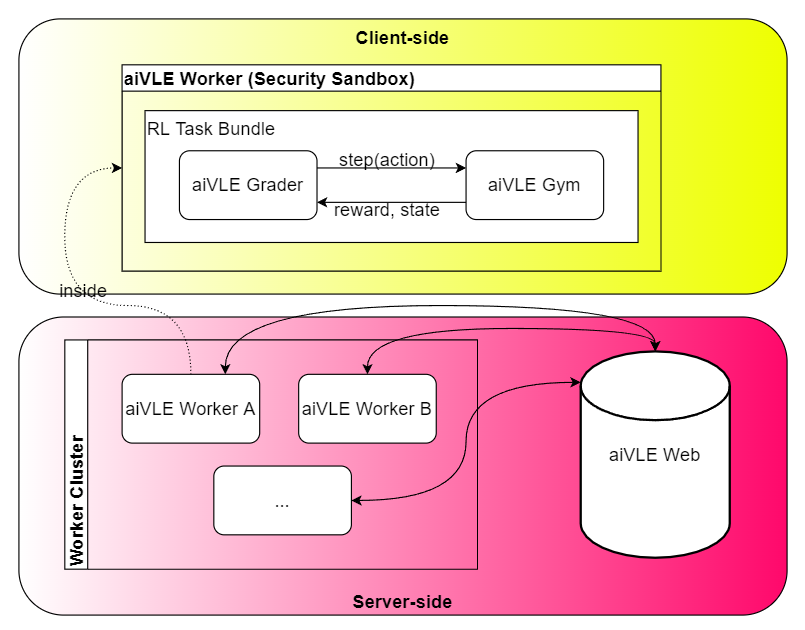
\includegraphics[width=0.9\textwidth]{images/architecture-overview.png}
    \caption{aiVLE 2.0 Architecture Overview}
    \label{fig:architecture-overview}
\end{figure}

In this chapter, we will discuss about the design and implementation of all these four components in detail, in the order of Gym, Grader, Worker and finally aiVLE Web. In fact, this is also the chronological order of development: the later components may have dependencies on earlier ones, and the earlier components generally\footnote{Strictly speaking, aiVLE Worker does not depend on aiVLE Web, but when it is used as a worker client on top of a security sandbox, although it will startup normally, without aiVLE Web to push evaluation jobs into the task queue, the worker client is meaningless. So we used ``generally'' here just to be precise.} do not depend on the later ones. For example, aiVLE Gym can be used as general-purpose multi-agent environment framework outside of the aiVLE 2.0 platform.

\section{aiVLE Gym - Separating Agents from Environment}
\label{ch:aivle-gym}
I have released a stable version of aiVLE Gym with all planned features implemented. \href{https://github.com/edu-ai/aivle-gym}{The source} consists of $\sim$1K lines of code, including several example environments and full documentation. The package is published to PyPI  (\href{https://test.pypi.org/project/aivle-gym}{https://test.pypi.org/project/aivle-gym}) so that aiVLE Gym can be installed and imported like any other Python package.

\subsection{Motivation}
aiVLE Gym makes multi-agent competition possible by separating agents from the environment. In a two-agent OpenAI Gym task, we write agent code as shown in Code~\ref{code:two-agent-example}:

\begin{code}
\begin{minted}[frame=lines,framesep=2mm,baselinestretch=1.2,bgcolor=LightGray,fontsize=\footnotesize,linenos]{python}
env = gym.make("PongDuel-v0") # Two-player Ping Pong game

for ep_i in range(100):
    done_n = [False for _ in range(env.n_agents)]
    ep_reward = 0
    obs_n = env.reset()
    env.render()
    while not all(done_n):
        action_0 = decide_0(obs_n[0], reward_n[0])
        action_1 = decide_1(obs_n[1], reward_n[1])
        action_n = [action_0, action_1]
        obs_n, reward_n, done_n, info = env.step(action_n)
        ep_reward += sum(reward_n)
        env.render()
    print('Episode #{} Reward: {}'.format(ep_i, ep_reward))

env.close()
\end{minted}
\captionof{listing}{OpenAI Gym agent example}
\label{code:two-agent-example}
\end{code}

Note that in a multi-agent scenario, \texttt{observation}, \texttt{reward} and \texttt{done} are all vectors - each element corresponds to one of the agents. Similarly, when you call \texttt{env.step()}, you should provide \texttt{action}s for every agent in this simulation. Such design is acceptable when we perform these multi-agent experiments offline. However, in a competition setting, when it comes to multi-agent tasks, you cannot make decisions for your opponent agents. Therefore, separating agents from the environment simulation is necessary. From the perspective of each agent, it is just like a single-agent environment – the only difference is that the environment is affected by actions taken by other agents as well. Figure~\ref{fig:opanai-gym-multi-arch} and Figure~\ref{fig:aivle-gym-multi-arch} show the architectural differences between \emph{OpenAI} Gym and \emph{aiVLE} Gym (each colored box represents a separate process; solid arrows represent inter-process or network communication):
\begin{figure}[H]
    \centering
    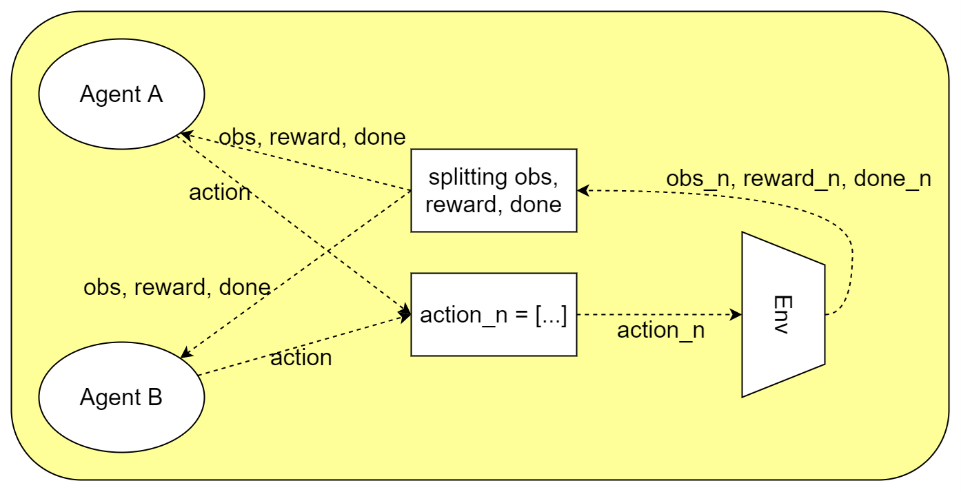
\includegraphics{images/opanai-gym-multi-arch.png}
    \caption{Multi-agent Architecture for OpenAI Gym}
    \label{fig:opanai-gym-multi-arch}
\end{figure}
\begin{figure}[H]
    \centering
    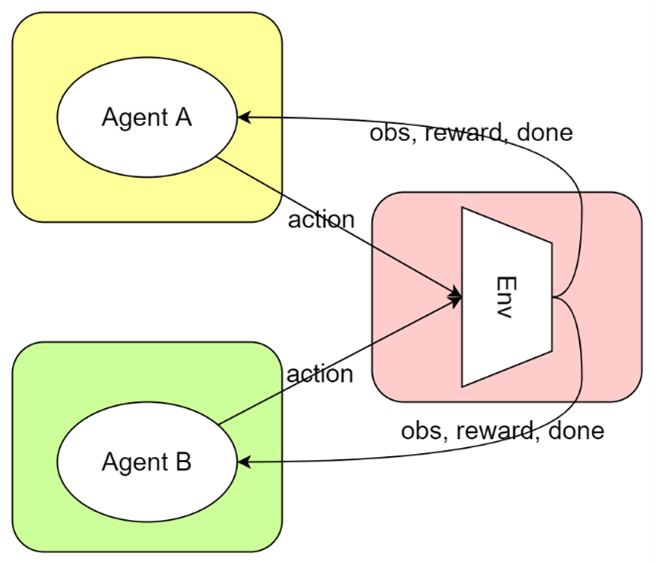
\includegraphics{images/aivle-gym-multi-arch.png}
    \caption{Multi-agent Architecture for aiVLE Gym}
    \label{fig:aivle-gym-multi-arch}
\end{figure}

\subsection{Design Goal}
Unless mentioned otherwise, all design goals in this chapter are achieved in the released implementation. 

The design goal of aiVLE Gym is to keep full compatibility with OpenAI Gym on the agent side. On the environment side, it lets you convert from existing OpenAI Gym environments with little adaptation. More specifically:

In single-agent case, on the agent side, traditional environment (simulation happens within agent process) and aiVLE environment (simulation happens outside of agent process) should be interchangeable. On the environment side, author can reuse existing OpenAI Gym compatible environment by implementing a serializer that serializes \texttt{action}, \texttt{observation}, and \texttt{info} to JSON compatible objects.

In multi-agent case, on the agent side, the APIs behaves just like normal single-agent OpenAI Gym environment. On the environment side, author can reuse existing ma-gym environment~\cite{magym} by implementing a serializer along with several metadata fields. 

\subsection{Agent-Environment Communication}
\label{ss:agent-env-communication}
Since agents and environment are separated, there needs to be an inter-process communication channel between them. aiVLE Gym uses a lightweight yet high-performance messaging library ZeroMQ~\cite{zeromq}, which has comprehensive support for many synchronous and asynchronous messaging patterns that are essential to this project. There are two primary challenges for multi-agent tasks when it comes to agent-environment communication:
\begin{enumerate}
    \item The judge should receive and respond to requests asynchronously - it needs to wait for all agents' actions before stepping forward in the environment, then decide what observations/rewards to respond to each of the agents.
    \item Certain operations (e.g., resetting the simulation) must be performed strictly once for each episode, but since each agent will initialize the episode on their own, judge-side will unavoidably receive multiple requests.
\end{enumerate}

To summarize, the judge-side environment needs to implement a ``barrier'' synchronization mechanism that not only realizes synchronous rendezvous of agent requests, but also performs additional tasks upon the ``first-comer'' and ``last-leaver''. 

Therefore, we propose the deterministic finite automaton (DFA) as shown in Figure~\ref{fig:aivle-gym-multi-dfa}:
\begin{figure}[H]
    \centering
    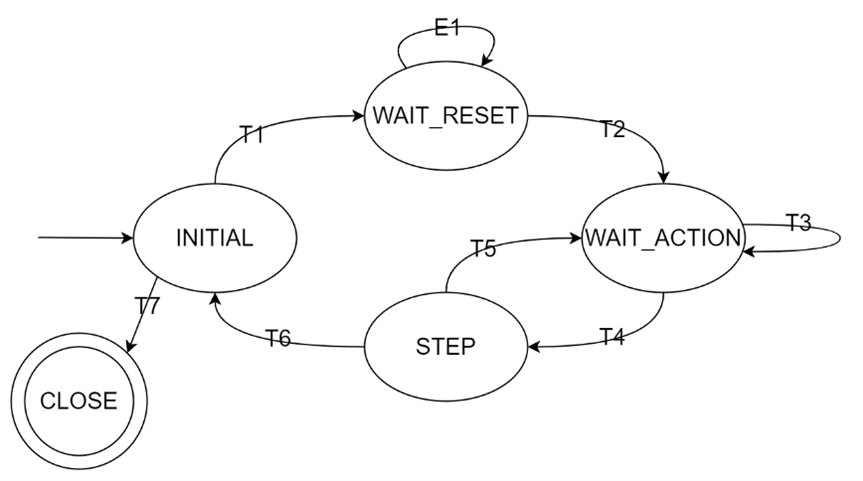
\includegraphics{images/aivle-gym-multi-dfa.png}
    \caption{aiVLE Gym Multi-agent Environment Communication Automaton}
    \label{fig:aivle-gym-multi-dfa}
\end{figure}

This DFA is key to keeping complicated communication details transparent to both agent and environment logic – both can write common synchronous code while the framework deals with the underlying asynchronous logic. Details of this DFA and messaging patterns involved can be found in the Appendix~\ref{as:aivle-gym_dfa}.

\section{aiVLE Grader - Evaluating Agents Using Test Suites}
\label{ch:aivle-grader}
I have released a stable version of aiVLE Grader with support for 1) OpenAI Gym, 2) aiVLE Gym single-agent, and 3) aiVLE Gym multi-agent environment. The codebase consists of $\sim$600 lines of framework code and $\sim$300 lines of example test suites for all three supported use cases. Similar to aiVLE Gym, the package is released to PyPI  (\href{https://test.pypi.org/project/aivle-grader/}{https://test.pypi.org/project/aivle-grader}) for in-production usage.

\subsection{Design Goal}
Unlike competitive programming style problems or machine learning prediction tasks, evaluating RL agents is much more complicated than comparing students’ output against a standard answer. Fortunately, with the common programming interfaces provided by OpenAI/aiVLE Gym, on top of them we may create a framework that standardizes/modularizes the initialization, execution, and conclusion of RL agent evaluation. The ultimate goal of this framework, when writing a grader for agents in any OpenAI/aiVLE Gym environment, is to:
\begin{enumerate}
    \item Make the built-in components so complete that for most use cases using built-in ones would be sufficient.
    \item Make each component self-contained without complicated inter-dependencies (i.e., following the single responsibility principle) when writing a custom component.
\end{enumerate}

\subsection{Key Abstractions}
There are three key abstractions to aiVLE Grader: \textit{agent}, \textit{evaluator}, and \textit{test case} as summarized in Figure~\ref{fig:aivle-grader-class}.

\begin{figure}[H]
    \centering
    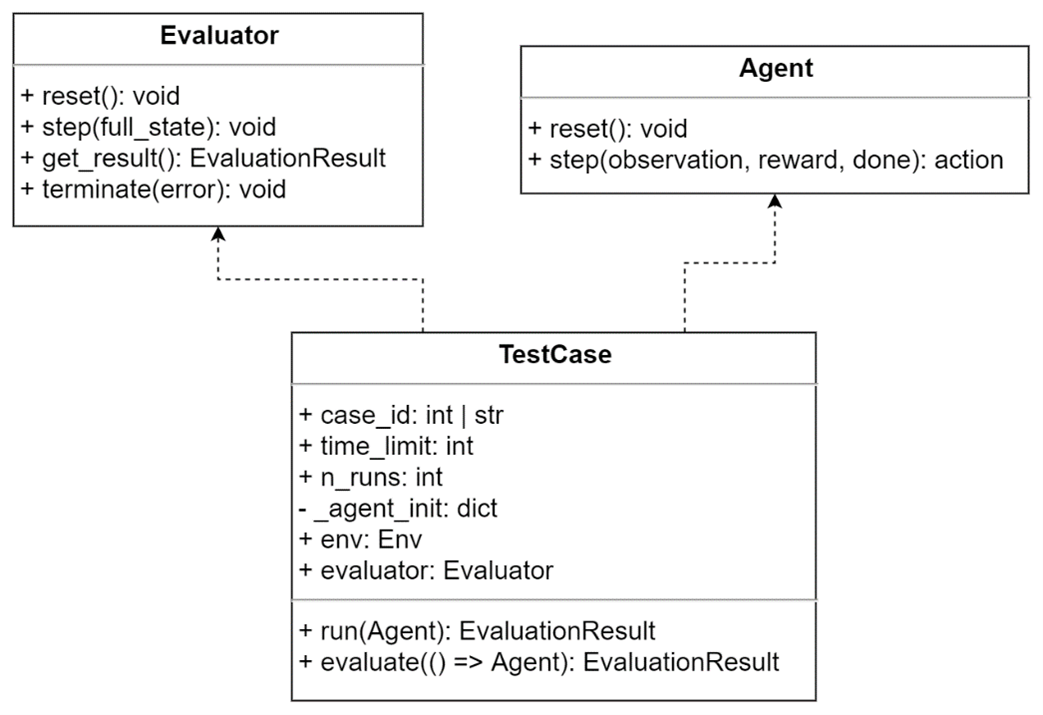
\includegraphics{images/aivle-grader-class.png}
    \caption{Class Diagram for aiVLE Grader}
    \label{fig:aivle-grader-class}
\end{figure}

\textit{Agent} only has two methods: \texttt{reset} to reset internal states, \texttt{step} to return an action from provided observation. It is flexible enough to allow agents to memorize the history, whilst restrictive enough to prohibit agents from modifying the inner-workings of the environment.

\textit{Evaluator} records the entire execution process and produces a score when the session terminates. It utilizes the common pattern of most RL tasks (see Figure~\ref{fig:obr-loop}): each session consists of many episodes, and each episode consists of many concrete steps. By inserting hook functions to these critical points, an evaluator practically records everything about the evaluation session. 

\textit{Test case} is a bootstrap for evaluation sessions. It wraps \textit{agent}, \textit{environment}, and \textit{evaluator} along with necessary initialization parameters into an object with one simple \texttt{evaluate} method. It also offloads certain chore (e.g., time limit) away from the user.

\section{aiVLE Worker - Secure and Scalable Grading Client}
\label{ch:aivle-worker}
I have released the second\footnote{Relative to the first stable version released during the first semester.} stable version of aiVLE Worker. The most significant upgrade from the second release is its resource awareness (see Section~\ref{ss:aivle-worker-resource-awareness}). It is validated on both CPU-only machines and GPU nodes with CUDA drivers (GTX 1050Ti for CUDA 10, RTX 3070 for CUDA 11). Moreover, it has been deployed and tested on several GPU nodes of the SoC Compute Cluster (see Section~\ref{s:deployment}). The codebase consists of $\sim$700 LoC, also with examples and detailed documentation. 

Unlike aiVLE Gym and Grader that are packages that are meant to be imported in other scripts, aiVLE Worker is a self-contained client that is runnable out-of-the-box. Thus aiVLE Worker is published to PyPI (\href{https://test.pypi.org/project/aivle-worker}{https://test.pypi.org/project/aivle-worker})  as a command-line tool. Users may install aiVLE Worker from PyPI and use it like any regular program (as shown in Figure~\ref{fig:aivle-worker-cli}).

\begin{figure}[H]
    \centering
    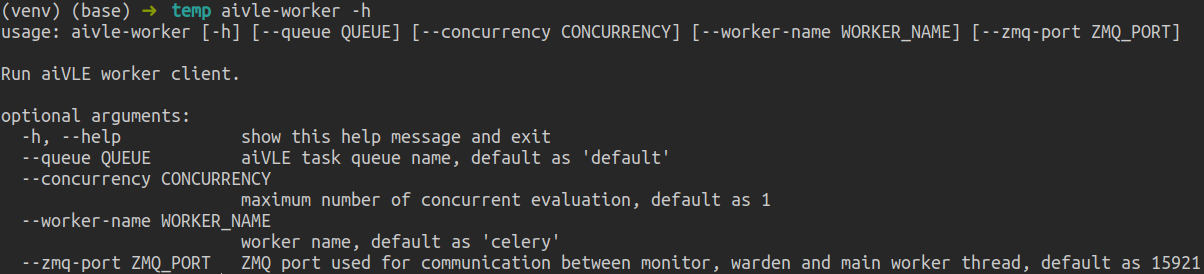
\includegraphics[width=\textwidth]{images/aivle-worker-cli.png}
    \caption{aiVLE Worker Command-line Interface}
    \label{fig:aivle-worker-cli}
\end{figure}

\subsection{Design Goal}
\label{ss:aivle-worker-design-goal}
For security, the implementation is expected to achieve:
\begin{enumerate}
    \item File access restriction: agent program should have no access to directories that may contain sensitive data (e.g., private keys), and should have read only access to files necessary for its execution (e.g., Python binary, dependencies, agent, and environment source code).
    \item Network restriction: agent program should have no access to the Internet. Otherwise, (1) it may benefit from extra computation resources; (2) it may send out confidential runtime details (e.g., configuration of simulation environment) that allow users to fine-tune their program; both of which make the competition unfair.
    \item Resource limit: agent program should be terminated and reported if it exceeds RAM limit, VRAM limit or time limit.
\end{enumerate}

For scalability, in addition to the task queue system that manages all worker nodes and distributes evaluation jobs fairly and efficiently to the workers (see Section~\ref{ch:aivle-web_highly-available-task-queue}), on the worker side, a client that requires little permission and setup would be extremely helpful. It benefits horizontal scalability because 1) adding new worker nodes is easier, 2) more machines can be used as worker nodes (e.g., shared GPU servers, programming lab PCs). Thus, what we expect from this solution are:
\begin{enumerate}
    \item Managed concurrency: it should be able to run as many evaluation jobs concurrently as the hardware resource permits, while being able to detect and terminate processes that consume excessive RAM/VRAM. For more details please refer to Section~\ref{ss:aivle-worker-resource-awareness}.
    \item Minimal permission requirement: if we have access to run the submission locally, the environment should be able to operate as a worker node (i.e., sudo is not required).
    \item Minimal dependency requirement: any Linux machine with Python should be able to run the worker client.
    \item Moderate overhead: compared to traditional OJ, aiVLE can trade some overhead (both startup and runtime) for absolute essentials like GPU support. However, to achieve a certain level of throughput, crazy warmup time like several minutes is still unacceptable.
\end{enumerate}

\subsection{Security Solution}
There are three mainstream security solutions for our consideration: 1) virtual machine (VM) such as Virtualbox, 2) container such as Docker/Podman, and 3) sandbox such as Firejail. The primary areas of interest are compared in Table~\ref{tab:security-solutions}\footnote{There are some caveats to the claims listed in this table. For more details please refer to Appendix~\ref{as:comparison-of-security-solutions}.}:

\begin{table}[H]
\centering
\begin{tabular}{|c|c|cc|c|}
\hline
\multirow{2}{*}{} & \textbf{VM} & \multicolumn{2}{c|}{\textbf{Container}} & \textbf{Sandbox} \\ \cline{2-5} 
 & VirtualBox & \multicolumn{1}{c|}{Docker} & Podman & Firejail \\ \hline
\textbf{Rootless} & No & \multicolumn{1}{c|}{Yes} & Yes & Yes \\ \hline
\textbf{Level of isolation} & Very high & \multicolumn{2}{c|}{High} & Medium \\ \hline
\textbf{Overhead} & High & \multicolumn{2}{c|}{Low} & None \\ \hline
\textbf{Startup time} & $\sim$15s & \multicolumn{2}{c|}{$\sim$3s} & $\sim$0.05s \\ \hline
\textbf{GPU support} & No & \multicolumn{2}{c|}{Yes, with NVIDIA container runtime} & Yes \\ \hline
\end{tabular}
\caption{Comparison of Mainstream Security Solutions}
\label{tab:security-solutions}
\end{table}

There are several must-haves for the candidate solution:

\begin{enumerate}
    \item GPU-support. Many recent RL algorithms are practically impossible to run without a GPU. This eliminates VM without PCI passthrough.
    \item Server needs to be shared. This eliminates VM with PCI passthrough as it requires exclusive access. This also eliminates Podman and Docker, as they prevent the GPU from being shared by any other container with root access.
\end{enumerate}

Therefore, Firejail is the only option left. I built a custom security profile to expose only the necessary file system and devices to processes inside the sandbox. I also used Firejail to impose CPU affinity and RAM usage limit on each sandbox.

\subsection{Resource Awareness}
\label{ss:aivle-worker-resource-awareness}
The architecture of aiVLE Worker's resource awareness is illustrated in Figure~\ref{fig:aivle-worker-resource-awareness-arch}. In the following subsections, we will discuss the objectives and design of related components, namely \texttt{monitor} and \texttt{warden} modules.

\begin{figure}[H]
    \centering
    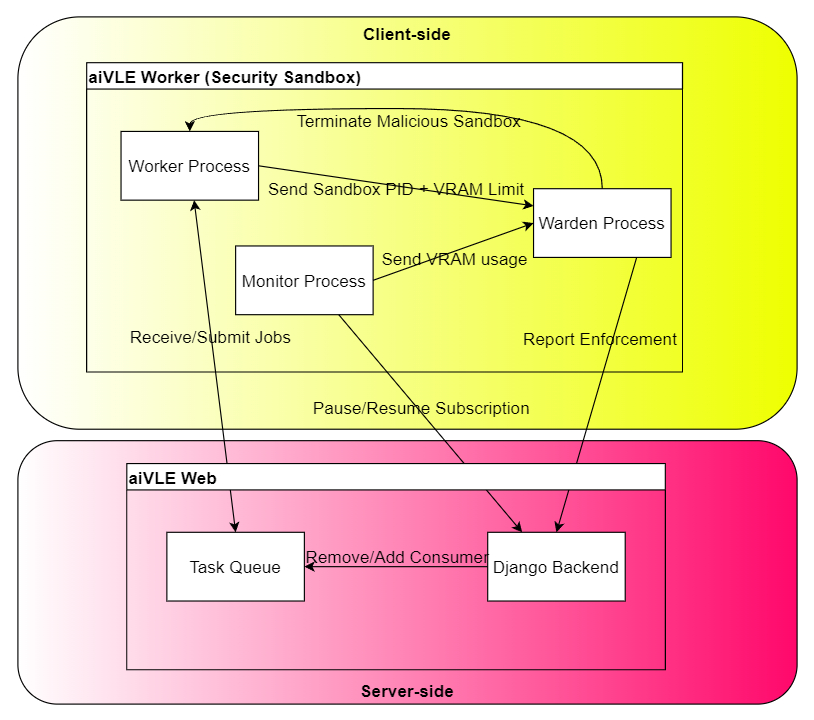
\includegraphics[width=0.8\textwidth]{images/aivle-worker-resource-awareness-arch.png}
    \caption{aiVLE Worker Resource Awareness Architecture}
    \label{fig:aivle-worker-resource-awareness-arch}
\end{figure}

\subsubsection{Resource Monitoring - \texttt{monitor} module}
\label{sss:monitor}
To achieve resource-sensitive load balancing as described in a later Section~\ref{ss:aivle-web-load-balancing}, and to enforce resource limit as described in Section~\ref{sss:warden}, we need to monitor CPU/GPU utilization and RAM/VRAM usage and take actions accordingly. Therefore we implement the \texttt{monitor} module inside aiVLE Worker that runs in parallel with the main worker process. The \texttt{monitor} module
\begin{enumerate}
    \item Monitors the system utilization periodically
    \item Controls the worker's task queue subscription according to prefetched threshold
    \item Sends monitoring metrics to the \texttt{warden} module to enable resource limit enforcement
\end{enumerate}

The first objective is achieved by the execution flow illustrated in Figure~\ref{fig:aivle-worker-monitor-flow} with the help of \href{https://pypi.org/project/psutil/}{\texttt{psutil}} for CPU/RAM monitoring and \href{https://github.com/fbcotter/py3nvml}{\texttt{py3nvml}} for GPU monitoring. The last objective involves inter-process communication that will be discussed later in detail with Figure~\ref{fig:aivle-worker-ipc}.

\begin{figure}[H]
    \centering
    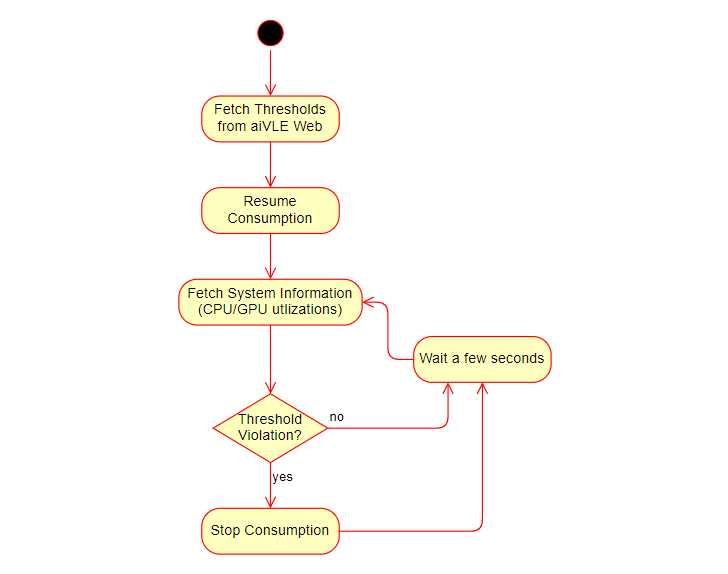
\includegraphics[width=0.45\textwidth]{images/aivle-worker-monitor-flow.png}
    \caption{Execution Flow of \texttt{monitor} module}
    \label{fig:aivle-worker-monitor-flow}
\end{figure}

Now we explain why the \texttt{monitor} module is also responsible for controlling the task queue subscription: due to the limitation of Celery (the distributed task queue library we used to build the evaluation subsystem), the subscription control is unidirectional. In other words, Celery does not allow the worker itself to pause \textbf{consuming} tasks - the worker can only \textbf{shutdown} itself entirely, and only the master server can pause \textbf{sending} tasks to a certain worker. So we have two possible designs: either sending monitoring metrics periodically to the master server and let the master server have full control, or make the workers fetch the threshold on startup and request the master server to pause whenever the threshold is violated. The second option is our obvious choice because it incurs much less communication overhead and a fixed, prefetch threshold works fine in our use case.

\subsubsection{Limit Enforcement - \texttt{warden} module}
\label{sss:warden}
The \texttt{warden} module is responsible for:
\begin{enumerate}
    \item Collecting task information from \texttt{worker} module
    \item Collecting system resource information from \texttt{monitor} module
    \item Terminating sandboxes that violates resource restrictions and report to aiVLE Web\footnote{We use ``master server'' and aiVLE Web interchangeably in the context of task queue because they run in the same Python monolithic server application.}
\end{enumerate}

Terminating sandboxes and reporting to aiVLE Web is as straightforward as killing the corresponding PID and making an HTTP request. What makes \texttt{warden}'s job challenging is its first two objectives: there are three modules that run in parallel: \texttt{worker}, \texttt{monitor} and \texttt{warden}. And they need to exchange information in order to collaborate. This is where ZeroMQ~\cite{zeromq} comes handy\footnote{...again, see Section~\ref{ss:agent-env-communication}}: only the worker knows the mapping from sandbox PID to task information (i.e., VRAM limit), and only the \texttt{monitor} knows the VRAM usage of each process. Both need to send their data to the \texttt{warden} process which oversees all running jobs and terminates jobs that violates restrictions. Figure~\ref{fig:aivle-worker-ipc} shows the inter-process communication among these three:

\begin{figure}[H]
    \centering
    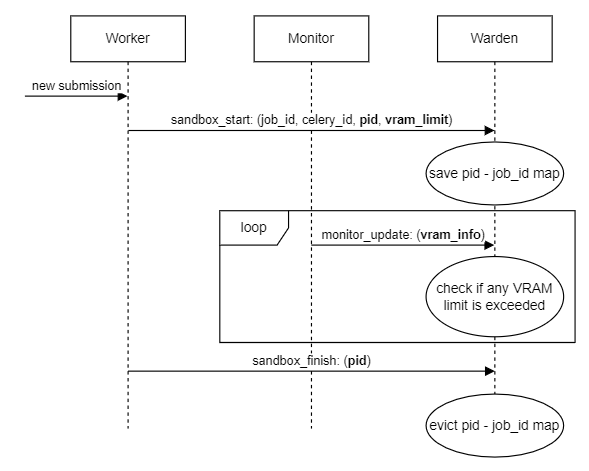
\includegraphics[width=0.8\textwidth]{images/aivle-worker-ipc.png}
    \caption{aiVLE Worker Inter-process Communication}
    \label{fig:aivle-worker-ipc}
\end{figure}

For \texttt{warden}'s case, every time it receives an update from \texttt{monitor}, it goes through the list of active sandboxes, queries the process hierarchy\footnote{This is necessary as most frameworks like PyTorch will spawn new processes for computation. Generally the process that is directly utilizing GPU is no longer the parent process. And there might be multiple processes in the same sandbox that consumes VRAM. By traversing the process tree recursively, we prevent intentional or unintentional attempts of ``downplaying'' the resource consumption of certain sandboxes.} to calculate the total VRAM usage of each sandbox, and finally checks if any sandbox needs to be terminated.

\section{aiVLE Web - AI competition platform}
\label{ch:aivle-web}
aiVLE Web consists of a Django backend that is $\sim$2.5K LoC and a React frontend that is $\sim$2K LoC. An active instance is deployed on the server and is accessible from \href{https://aivle.leotan.cn/}{https://aivle.leotan.cn/} (frontend) and \href{https://aivle-api.leotan.cn/}{https://aivle-api.leotan.cn/} (API and admin panel). Figure~\ref{fig:aivle-web-frontend-screenshot} shows a few screenshots of the React frontend. Do note that we used mobile-sized screenshots due to limited space, but the design is responsive (i.e., it adapts to different screen sizes).

\begin{figure}[H]
    \centering
    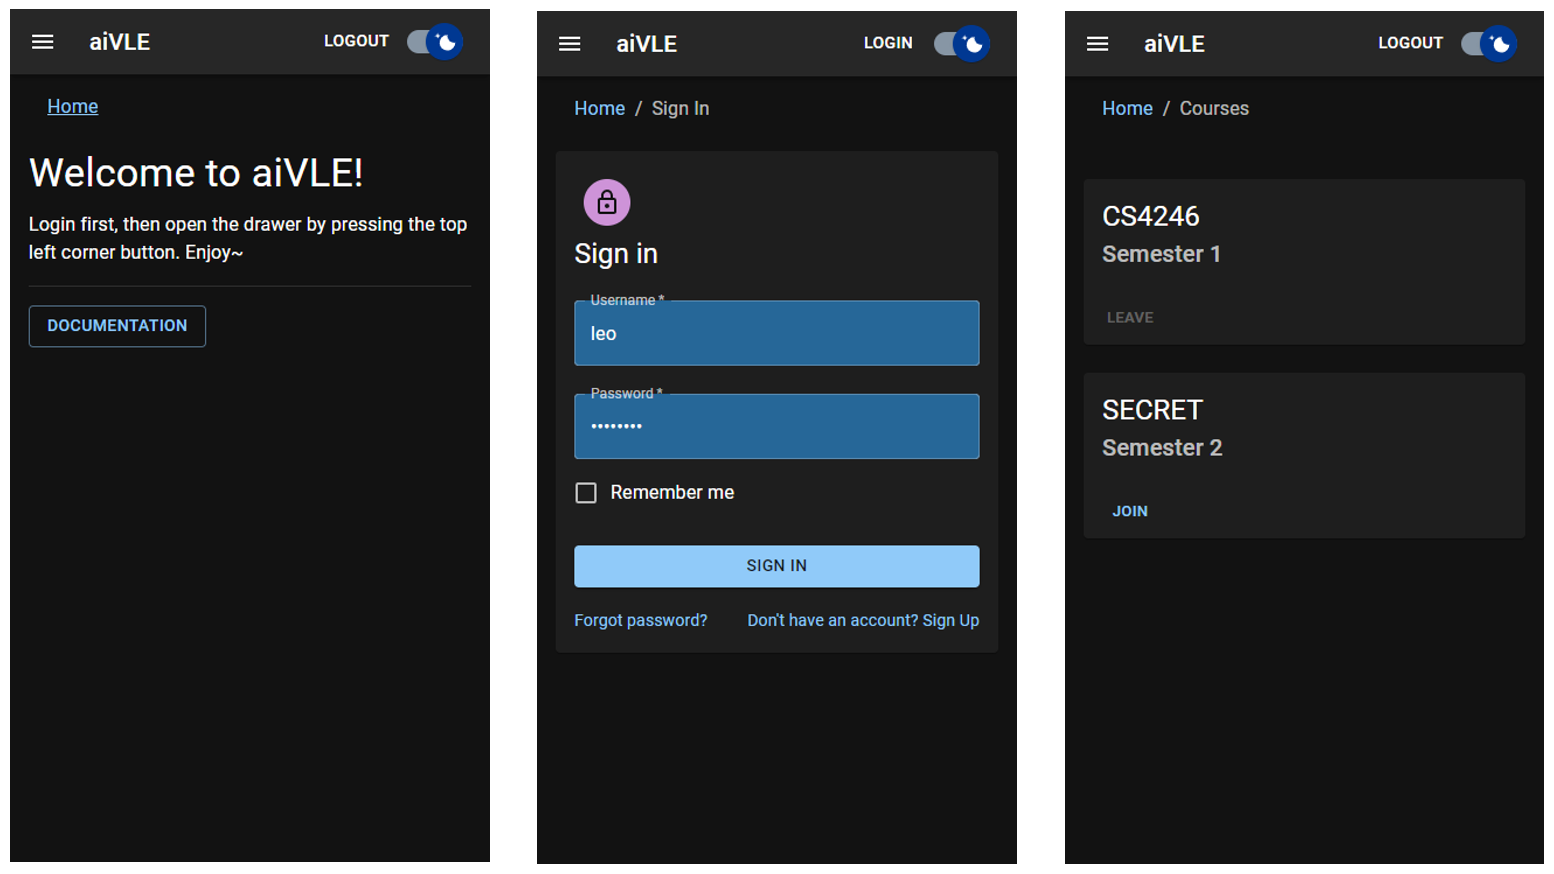
\includegraphics[width=\textwidth]{images/aivle-web-frontend-screenshot.png}
    \caption{aiVLE Web Frontend Screenshots}
    \label{fig:aivle-web-frontend-screenshot}
\end{figure}

\subsection{Design Goal}
There are three primary considerations to the design of aiVLE web: extensibility, scalability, and usability. 

\textbf{Extensibility} means the architecture should be flexible enough for future upgrades including but not limited to multi-agent task competition. Due to space limit we refrain from discussing the software engineering choices that are in favor of extensibility, but you may take a sneak peek at how to extend the existing system from Appendix~\ref{appendix:aivle-web_matchmaking}: \nameref{appendix:aivle-web_matchmaking}.

\textbf{Scalability} means the platform should be able to spread the evaluation workload, which is obviously the most computationally heavy task, over many worker machines. We will discuss this objective in detail with 1) highly available and fault tolerant task queue (Section~\ref{ch:aivle-web_highly-available-task-queue}) and 2) resource-sensitive load balancing (Section~\ref{ss:aivle-web-load-balancing}).

\textbf{Usability} means the platform should provide all the features the users (e.g., CS4246 teaching team) need for a successful semester of teaching. While there are many features we could discuss, also due to space limit, we pick the role-based permission model (Section~\ref{ss:aivle-web-permission-model}) as an typical example of how we carefully balance complexity and flexibility during the development process.

\subsection{Highly Available and Fault Tolerant Task Queue}
\label{ch:aivle-web_highly-available-task-queue}
This is a continuation of \hyperref[ss:aivle-worker-design-goal]{scalability of (grading) workers} (Section~\ref{ss:aivle-worker-design-goal}). In the section for aiVLE worker, we addressed the problem of running the worker on as many computers as possible with as little configuration/permission as possible. Here we address the problem of 1) coordinating the communication between the workers and the backend server, and 2) distributing grading tasks to the workers efficiently for shorter waiting time and higher resource utilization.
\subsubsection{The Problem}
In aiVLE 1.0, there was no concept of ``task queue''. All pending tasks are stored in the DB with the status ``QUEUED''. Communication between the worker (or runner as per the term used by original author) and server is \textit{half-duplex by polling}. In other words, the worker makes \textbf{periodic} requests to the server for new ungraded submissions:
\begin{figure}[H]
    \centering
    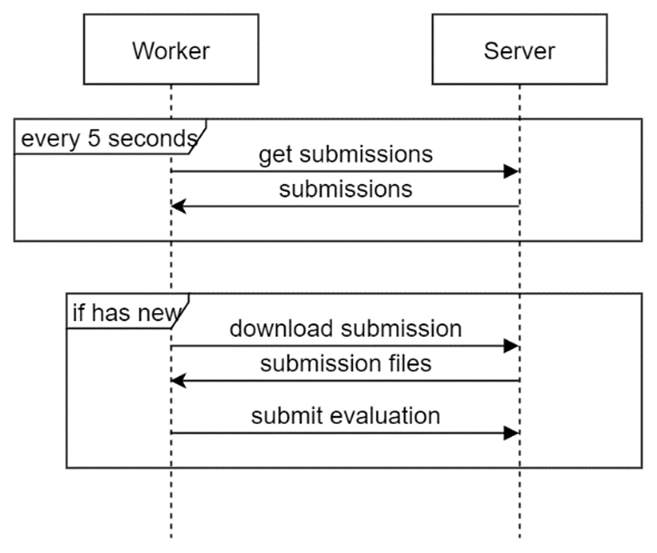
\includegraphics{images/aivle-web-old-task-queue.png}
    \caption{Old aiVLE “Task Queue”}
    \label{fig:aivle-web-old-task-queue}
\end{figure}
There are three critical limitations to this approach:
\begin{enumerate}
    \item Worker-side polling does not scale well: there is zero mechanism in orchestrating the timing and order of workers polling the server for new jobs. The severity of possible traffic spike (i.e., many workers poll the server at the same time due to lack of coordination) increases linearly with the number of worker nodes.
    \item Race condition: if two worker pull submissions at the same time, both will get the same ungraded submission. Such redundant work will get more significant with more worker nodes, which hurts the overall efficiency of the worker cluster.
    \item No concurrency on each worker\footnote{In the actual use of aiVLE 1.0, we run multiple worker clients on the same machine for disguised concurrency. Besides the inconvenience of manually starting multiple worker clients, this approach makes managing resources difficult as each client runs without knowing the existence of others even if they are on the same machine.\label{fn:worker-disguised-concurrency}}: each individual worker only polls for new job when it has no submission to grade. In other words, each worker can only grade one submission at a time.
    \item No load balancing: the backend has no control over which worker grades which submission, therefore load balancing is virtually impossible
\end{enumerate}

\subsubsection{The Solution}
Similar to the idea of extracting the responsibility of data storage/management into a separate database backend, we delegate the messaging tasks to a message queue (MQ). Conceptually, message queue enables asynchronous communication between clients (who submit tasks) and workers (who finish tasks). As for implementing the concept in our Python web application, we used \href{https://docs.celeryq.dev/en/stable/}{Celery} framework with \href{https://www.rabbitmq.com/}{RabbitMQ} message queue broker/backend. Figure~\ref{fig:aivle-web-mq} illustrates how the MQ-based task queue works:

\begin{figure}[H]
    \centering
    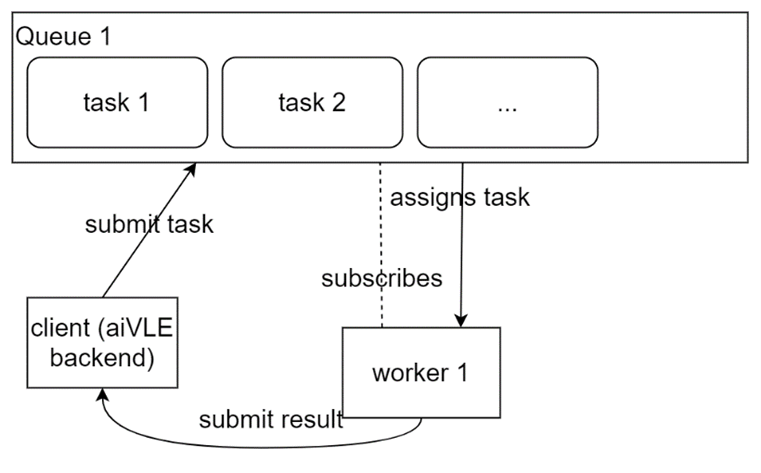
\includegraphics{images/aivle-web-mq.png}
    \caption{Message Queue Based Task Queue}
    \label{fig:aivle-web-mq}
\end{figure}

Every worker listens to one or more ``queues'', where the message broker is responsible for allocating tasks fairly among workers in each queue. When an evaluation job comes, aiVLE backend will submit the job to an appropriate queue (i.e., private queue if user has dedicated workers available, otherwise public CPU/GPU queue according to task specification) and wait for the assigned worker to submit evaluation result. The task will remain in the queue until it is processed (i.e., message queue is persistent). A randomly generated task ID is used to authenticate worker's submission – only the worker whom the broker assigned the task to will have this ID. This approach not only reduces the number of requests to be $O(n)$ where $n$ is the number of evaluation jobs, but also ensures fair distribution of tasks among workers. Moreover, we also benefit from other standard features of message queue such as automatic retry and heartbeat checks.

\subsection{Resource-sensitive Load Balancing}
\label{ss:aivle-web-load-balancing}
By using message queue for task distribution, we already have some primitive load balancing - Celery with RabbitMQ backend by default dispatches messages to all consumers in round-robin style, therefore all consumers are expected to consume the same number of tasks from the same queue over a fixed period of time. Although this is a huge improvement over no load balancing at all, from some stress testing using real-world workload, we find it necessary to take system load into consideration. Specifically, the primitive method of load balancing by number of tasks works poorly when certain tasks are much more resource intensive. For example, assume both worker A and worker B receive 5 submissions, but the ones for worker A consumes 30\% of total VRAM while the ones for worker B takes only 10\% of total VRAM. There are two serious implications in this imaginary scenario:
\begin{enumerate}
    \item \textbf{Unfairness}: suppose the worker is configured to run at most 8 concurrent evaluations, the fourth and fifth submissions arriving at worker A will not have sufficient VRAM. They will likely receive runtime errors which are entirely ours to blame.
    \item \textbf{Inefficiency}: suppose the task queue is configured to automatically retry the failed job by putting a new evaluation job into the same queue, since worker A is still accepting submissions, the retry attempt may take additional fails to finally arrive at worker B.
\end{enumerate}

The key to solving such unwanted behavior is 1) to monitor the available system resources, 2) to stop processing new tasks when the available resources fall below certain thresholds. Most of the heavy-lifting is handled on the worker side (see Section~\ref{ss:aivle-worker-resource-awareness}). As for aiVLE Web, it merely uses \texttt{add\_consumer} and \texttt{cancel\_consumer} Celery APIs for resuming and pausing consuming respectively. Nevertheless, there are two points to note in this solution:

\begin{enumerate}
    \item It does not cancel already running jobs. Instead, it only stops dispatching new tasks to the worker where the threshold is met. This behavior is acceptable in our case since we only need to promise students with a certain amount of resources to run their submissions. And our solution guarantees\footnote{Technically speaking, this guarantee does not hold between two checks on system information, but we can easily reduce the impact by performing the check more frequently. In our experience, one second interval is more than enough.} the promised amount of CPU/RAM/VRAM at the beginning of any evaluation job.
    \item It does not balance the resource utilization among all workers. \texttt{cancel\_consumer} simply removes the worker from the list of consumers to dispatch tasks to. To achieve resource utilization balance, aiVLE Web needs to understand each worker's utilization in real-time and dispatch tasks accordingly. We think the overhead (i.e., network traffic for reporting utilization data) and complexity (i.e., load balancing algorithm) of this design significantly outweighs the potential benefits.
\end{enumerate}

Besides addressing the previously mentioned two serious implications, surprisingly, resource-sensitive load balancing greatly increases the system utilization. As mentioned in Footnote~\ref{fn:worker-disguised-concurrency}, without resource awareness, aiVLE 1.0 could only achieve disguised concurrency by running multiple worker clients on the same machine. To ensure the machines will not be overloaded, we could only ``play it safe'' by always under-utilizing the resources. In fact, the current configuration of aiVLE 1.0 only allows 3 concurrent evaluations, resulting in an average of $\sim30\%$ of volatile GPU usage. In comparison, as we will show later in Section~\ref{ss:load-balancing-exp-results}, we can achieve up to $>90\%$ GPU utilization rate, and with the later introduced resource-sensitive load balancing, overloading the system is no longer a concern. This translates to roughly three times\footnote{In real world use you might not want to set the threshold to be as high as 90\%, but even with a conservative 80\% threshold the improvement is still very significant.} of a performance improvement.

\subsection{Role-based Permission Model}
\label{ss:aivle-web-permission-model}
In Django we have two major types of permission model: per-model permission (built-in authentication system) and per-object permission (\href{https://github.com/django-guardian/django-guardian}{django-guardian}). Per-model permission means the finest granularity is model-level, that is we may only check if the user has read/write/edit/delete access to the model. Per-object permission is the finest granularity possible as we can establish arbitrary permission between any object and any user. In fact, the worst possible space complexity is $O(mnk)$ where $m$ is the number of objects, $n$ is the number of users and $k$ is the number of permissions.

In our use case, model-based permission is too coarse-grained: a student should only be able to view the tasks in the course he/she enrolled in, rather than all the tasks available on the platform. On the other hand, object-based permission is too overkill: there might be hundreds of thousands of job records in the database, storing each user's permission to each job record is simply too wasteful\footnote{This can be avoided by properly configuring django-guardian, but its flexibility does allow arbitrary permission on any object as mentioned earlier. In fact, if we restrict django-guardian to avoid such wasteful behavior, we essentially have the soon-to-be-discussed role-based permission model.}. Therefore, we propose a solution that is the sweet spot between the two extremes: role-based permission model.

The entity relationship diagram of aiVLE Web is illustrated in Figure~\ref{fig:aivle-web-er-diagram}:
\begin{figure}[H]
    \centering
    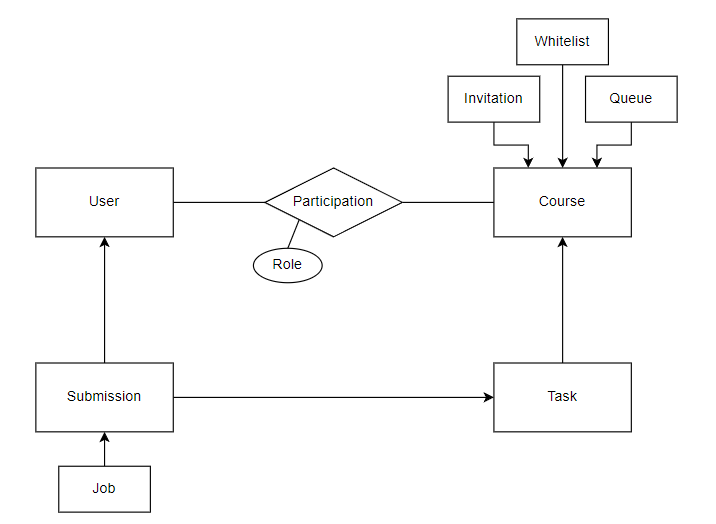
\includegraphics[width=0.8\textwidth]{images/aivle-web-er-diagram.png}
    \caption{aiVLE Web Entity Relationship Diagram}
    \label{fig:aivle-web-er-diagram}
\end{figure}

In the relational entity Participation, we record the ``role'' of the User in a Course. Possible roles\footnote{Note that a user can have different roles in different courses. And superuser who has access to absolutely everything is out of discussion here.} (as defined in \texttt{app.model.participation}) are: administrator (ADM), lecturer (LEC), teaching assistant (TA), student (STU) and guest (GUE).

The idea of role-based permission model is centered around one's role in the corresponding course: to determine one's access to any object, we first find the object's related course, then check if the user has access to this object in the context of this related course. For example, if we need to know if the user has view access to a certain \texttt{Job}, we can follow the arrows in the diagram: Job $\to$ Submission $\to$ Task $\to$ Course $\to$ Participation $\to$ User to find the corresponding role\footnote{The utility function \texttt{has\_perm} automatically queries the role given the course and the user, so its argument is the course instead of the role.}, and check if this role has \texttt{job.view} permission according to the permission lookup table (see Table~\ref{tab:aivle-web-permission-table}).

By introducing the \texttt{Participation} relational entity and \texttt{has\_perm(course, user, permission)} utility function, we compressed the worst case $O(mnk)$ space complexity to $O(nk)$ and it is a significant improvement. In reality the number of objects $m$ significantly outweighs the number of users $n$ or permissions $k$. We can summarize different roles' access (as defined in aiVLE.settings.ROLES) using a permission matrix in Table~\ref{tab:aivle-web-permission-table}:

\begin{table}[H]
\centering
\begin{tabular}{|c|l|l|l|l|l|l|}
\hline
\multicolumn{1}{|l|}{} &  & Admin & Lecturer & TA & Student & Guest \\ \hline
\multirow{5}{*}{Task} & View opened tasks & x & x & x & x & x \\ \cline{2-7} 
 & View all tasks & x & x & x &  &  \\ \cline{2-7} 
 & Add task & x & x &  &  &  \\ \cline{2-7} 
 & Edit task & x & x & x &  &  \\ \cline{2-7} 
 & Delete task & x & x &  &  &  \\ \hline
\multirow{4}{*}{Submission} & View own submissions & x & x & x & x &  \\ \cline{2-7} 
 & View all submissions & x & x & x &  &  \\ \cline{2-7} 
 & Add submission (under own name) & x & x & x & x &  \\ \cline{2-7} 
 & Download submission & x & x & x &  &  \\ \hline
\end{tabular}
\caption{Partial Permission Lookup Table}
\label{tab:aivle-web-permission-table}
\end{table}